\documentclass{article}
\usepackage[T1]{fontenc} % add special characters (e.g., umlaute)
\usepackage[utf8]{inputenc} % set utf-8 as default input encoding
\usepackage{ismir,amsmath,cite,url}
\usepackage{graphicx,color}
\usepackage{epigraph}

% UNCOMMENT THE TWO LINES BELOW TO SEE LINE NUMBERS. I think it is better without the line numbers.
% \usepackage{lineno}
% \linenumbers

\title{Chiptune Extension and Generation using Markov chains}

% Three addresses
% --------------
\threeauthors
  {Oscar Sandford} {University of Victoria \\ {\tt oscarsandford@uvic.ca}}
  {Colson Demedeiros} {University of Victoria \\ {\tt cdemedeiros@uvic.ca}}
  {Jae Park} {University of Victoria \\ {\tt jaehyunpark@uvic.ca}}

\sloppy
\begin{document}
\maketitle

% \epigraph{Do we understand what we are doing?}{\textit{George Tzanetakis}}

\begin{abstract}
Music generation is a well-studied field. Previous attempts at music generation have succeeded in replicating training tracks using various methods involving complex 
time inference models. In this paper we show that simple, but appropriately designed, first and $k$-order Markov models are a sufficient enough machinery to both 
replicate and generate classic 8-bit video game music.\footnote{This abstract will be expounded in time, pending study completion and results organized.}
\end{abstract}

\section{Introduction}
Music is typically constructed by humans, for humans. However, machines are becoming more adept at revealing patterns in the way musicians craft their chords. 
This enables humans to create their own music, and then let the machine take over the task of composer. Our project implements models for simple 8-bit music 
generation using temporal inference techniques. In the following section, we explore previous implementations and existing literature regarding music generation. 
Later, we will present techniques for designing generative Markov models to extend music as well as create derivative musical works.

\section{Background}
\subsection{Chiptunes}
Chiptunes, also called 8-bit music, originated in the 1980s and the 1990s, when hardware limitations for video game devices allowed only simple waveforms such as 
square, triangle, and saw waves \cite{pop_chiptunes}.  As a result, the necessary waveforms can be composed relatively easy in a computer. 

Some examples of chiptunes come from various classic video games, including Super Mario Brothers \cite{kondo_2009}, Undertale \cite{fox_2017} and 
Legend of Zelda \cite{nakatsuka_2009}.

\subsection{Markov Chains}
Markov chains model a \emph{sequence of states}.\footnote{In this study, we formulate the states as piano notes. Exact specification is revealed later.} Changes from 
one state to another are called \emph{transitions} \cite{markov_survey}. If one is to predict by hand which state will come next, given a certain state sequence, one might 
consider patterns in the sequence up until this point. That is, the probability distribution of a current state at time $t$ is conditioned on all the previous states.

\begin{align*}
  P(X_t | X_{0:t-1})
\end{align*}

However, the number of previous states to consider from the beginning will be unbounded as the number of states grows. To this end, we use the \textbf{Markov assumption} that 
the current state is only dependent on a fixed number of $k$ previous states \cite{russell_norvig_2022}. This is the backbone of the so-called Markov processes (also called 
Markov chains). 

\begin{align*}
  P(X_t | X_{0:t-1}) = P(X_t | X_{t-k:t-1})
\end{align*}

The variable $k$ reflects what is called the \textbf{order} of the Markov process. First-order Markov processes have the current state depend \emph{only} on the previous 
state, making transitions completely independent from state before the one directly before the curren state \cite{russell_norvig_2022}.

Any given set of $k$ states can have an arbitrary number of possible next states, each assigned its own transition probability. The sum of the transition probabilities 
for each option must sum to 1 \cite{markov_construct}. 

Markov chains are generative models, consisting of a set of states of size $N$. First-order models use a transition matrix of size $N\times N$ to store transition 
probabilities, but transition matrices for higher-order (i.e. $k>1$) processes may be larger.

Hidden Markov models incorporate "hidden" states. Consider an unstable coin that has two states: fair (50-50) or biased (90\% tails) \cite{hmms}. One cannot necessarily 
discern the coin's state simply from appearance, but we can infer the state through observations "emitted" by the hidden state. This variation on the Markov model is very 
useful, as we will see in the following section on related works. 

\section{Related Work}
\subsection{Inference Models}
Yanchenko and Mukherjee explored the use of Hidden Markov Models (HMMs) to compose classical music, finding proficiency in generating consonant harmonies, but 
lacking melodic progression \cite{yanchenko_2017}. Indeed, the models were found to learn the harmonic hidden states quite well, in some cases leading to overfitting. 
HMMs have also found use in chorale harmonization, where a given observable melody uses inference to derive hidden harmonies to complement it \cite{allan_2005}, as well 
as drum beat detection in polyphonic music \cite{drum_detection}. 

Walter and Van Der Merwe's methods involve representing the chord duration, chord progression, and rhythm progression with first or higher-order Markov chains, whereas 
the overlaying melodic arc is represented by a HMM \cite{walter_2011}. This separation works well to reduce the processing power needed for music generation, but the 
independent learning of each component leads to less cohesive compositions. Generating music is generally done by sampling a statistical model \cite{conklin_2003}.
However, we want to create music that does not only simply replicate the training data, but also creates cohesive pieces in a more natural way. 

Shapiro and Huber's approach to music generation simply uses Markov chains, no hidden states \cite{shapiro_huber_2021}. In their work, the states represent sound 
objects with attributes such as pitch, octave, and duration. Their results show that human-composed pieces can be closely replicated using the simpler Markov chains. 
Further, they have attached their implementation in their paper. We will consider this work when constructing our own implementation.

Corrêa and Jungling suggest using Markov chains of different orders to predict classical music. By using stochastic models to analyze different classcal songs and styles,
the computer can even capture subtle and intuitive features such as style of the composer. Although this paper focuses on classical music and its prediction, the authors 
stress that its application to other music genres should be straightforward \cite{correa_jungling_small_2020}. 
The only requirement is a MIDI file with a good quality, as it should be used for Markov chains that can properly estimate the music's pattern.

\subsection{Data Format}
The papers previously mentioned use the MIDI file format to write digital music. This format appears to be the standard for digital music creation \cite{midi_format}. 
One of MIDI's drawbacks is that it cannot store vocals \cite{cataltepe_2007}. This is of no concern to us, as we will only be attempting to generate instrumental 
compositions. Additionally, successful approaches to melody extraction from MIDI files \cite{ozcan_2005} make assurances that this will be an adequate medium for the 
music our models will generate. MusicXML is a standard file format for storing sheet music, just as MP3 is for recordings \cite{musicxml_2022}. Both are commonly used 
standards, and after experimenting with MusicXML for input data, we decided to use MIDI instead.

We decided to map MIDI to RTTTL (RingTone Text Transfer Language) notes. RTTTL is format used to specify ringtones for Nokia phones, and is composed of a comma-separated 
string of notes of a given format \cite{rtttl_spec}. RTTTL is perfect for this study because notes (states) come one after another, in a sequence.

\section{Initial Approach}
After considering the differences between HMMs and simpler Markov models, we decided to design our generator as a $k$-order Markov process without hidden states, 
since these methods have seen success in recent works \cite{shapiro_huber_2021,correa_jungling_small_2020}. 

Initially, we had two designs in mind. The first approach involved representing a song with a single chain of sound object states, including pitch, octave, duration, 
and other attributes. An alternative used $m$ separate $k$-order Markov processes, one for each key on a piano used in the song. It would be prudent to consider extending 
the order of the processes in this case, in order to capture the musical patterns more clearly. First-order probabilistic transitions will inevitably make the generated 
notes very random. Extending the process order would alleviate the generative faults coming from independently trained Markov chains.

\subsection{Timeline}
We expect to have 3 milestones for this project:
\begin{enumerate}
  \item \textbf{Milestone 1} (February 18th): Convert music to MusicXML files using AnthemScore. Devise sound object structure for Markov states or other architecture. 
  Write a parser to transform the MusicXML data to sound objects. 
  \item \textbf{Milestone 2} (March 21st): Apply Markov chain algorithm to the music samples in order to train the model. We plan to refer to various works that we found.
  By this point, our models should be able to replicate the music tracks given as input. By this point our program will be able to extend music.
  \item \textbf{Milestone 3} (April 7th): Tweak the models to generate more original variations. Enhance the quality of the music. Possibly a GUI for aesthetics as well, 
  if time permits.
\end{enumerate}

\subsection{Task Delegation}
In order to figure out the best approach and gather a plethora of sources, each team member researched various sources related to music data parsing and music generation, 
from theoretical papers to Python libraries. Colson and Jae found classic 8-bit tracks for use training and testing our models. Oscar set up a GitHub repository to include 
written work as well as source code, and made outlines for the final report. Colson would then be responsible for finding mumsic, and designing a parser to turn notes into 
data. Jae and Oscar would work on figuring out the best state attributes and designing the generative Markov models. 

\subsection{Resources}
\subsubsection{Tools}
Stacher\footnote{https://stacher.io} is a frontend GUI for YT-DLP, which is a command line downloader that can be installed for converting Youtube videos to MP3 files.
While YT-DLP works just fine, Stacher makes it very easy to convert YouTube links to various file formats (MP3, WAV, AAC, etc.) and save them on your current device. This 
is software we could use to get the songs as MP3 files saved and put into AnthemScore to be converted into XML files.

AnthemScore\footnote{https://www.lunaverus.com/} is a music transcription software that converts WAV, MP3, and other audio formats into sheet music using an advanced 
neural network. The sheet music can then be exported to various other formats such as PDF, MIDI, or XML. The main use of this software is to easily obtain XML files that 
we would have used for data in the Markov chains. While AnthemScore is a great tool to aquire relatively true XML files of songs, the artificial intelligence that 
powers it does occasionally miss notes. What this means for us is that without changing the notes that are detected and placed by the AnthemScore software, it may miss notes 
or sounds that exist within the original song. Despite this, as long as it is mostly accurate and the majority of notes are in place, it shouldn't affect the overall process 
of the project. We avoided songs that don't transform accurately into MusicXML. Preliminary coding will be done in Jupyter Notebooks using Python. 


\section{Final Approach}
\subsection{Initial Steps \& Restrictions}
The first step we took was the decision to move away from the MusicXML format we started with, for a couple of reasons. For one, it required a software called AnthemScore, 
which is a paid service that works by converting MP3 files to MusicXML format. We had originally downloaded it with a one month free trial, and had intended to find a 
selection of songs in that time, and convert them to MusicXML immediately. We decided that this approach was not extensible, as any future progress using this method would 
require the software again to access new data. From here, we landed on MIDI files to use as data instead, as the existing Mido Python library makes accessing the files and 
data easy. This also removed Stacher, the software we had used to turn YouTube links into MP3, as a requirement.

Another thing we had to consider was the complexity of the MIDI files we used as data. For the most part, the code we wrote to interpret the MIDI file data is quite simple, 
capturing things like the time signature, key signature, tempo, as well as the tracks turned into a list of notes. MIDI files can be quite complex, using things like 
system exclusive messages, control change messages, and more. 

The second issue was related to the creators of the MIDI tracks, and how they decided to implement simultaneous notes. Due to the nature of the RTTTL format, notes and rests 
play in sequence, from start to finish. We intended to have each MIDI track be a different part of the song, which would then each have its own RTTTL track that would be 
analyzed. Unfortunately, track creators can also have notes play simultaneously in one MIDI track by having a new note on message at $time = 0$ following another note on message 
of a different note. For these kinds of tracks, we simply have to drop one of the notes that is played, since we cannot easily separate them, and we cannot have them play 
simultaneously in RTTTL format. This, along with the more unique MIDI messages present in some songs, are the two main restrictions to our implementation and the tracks we 
have used as data. \\

% \frame{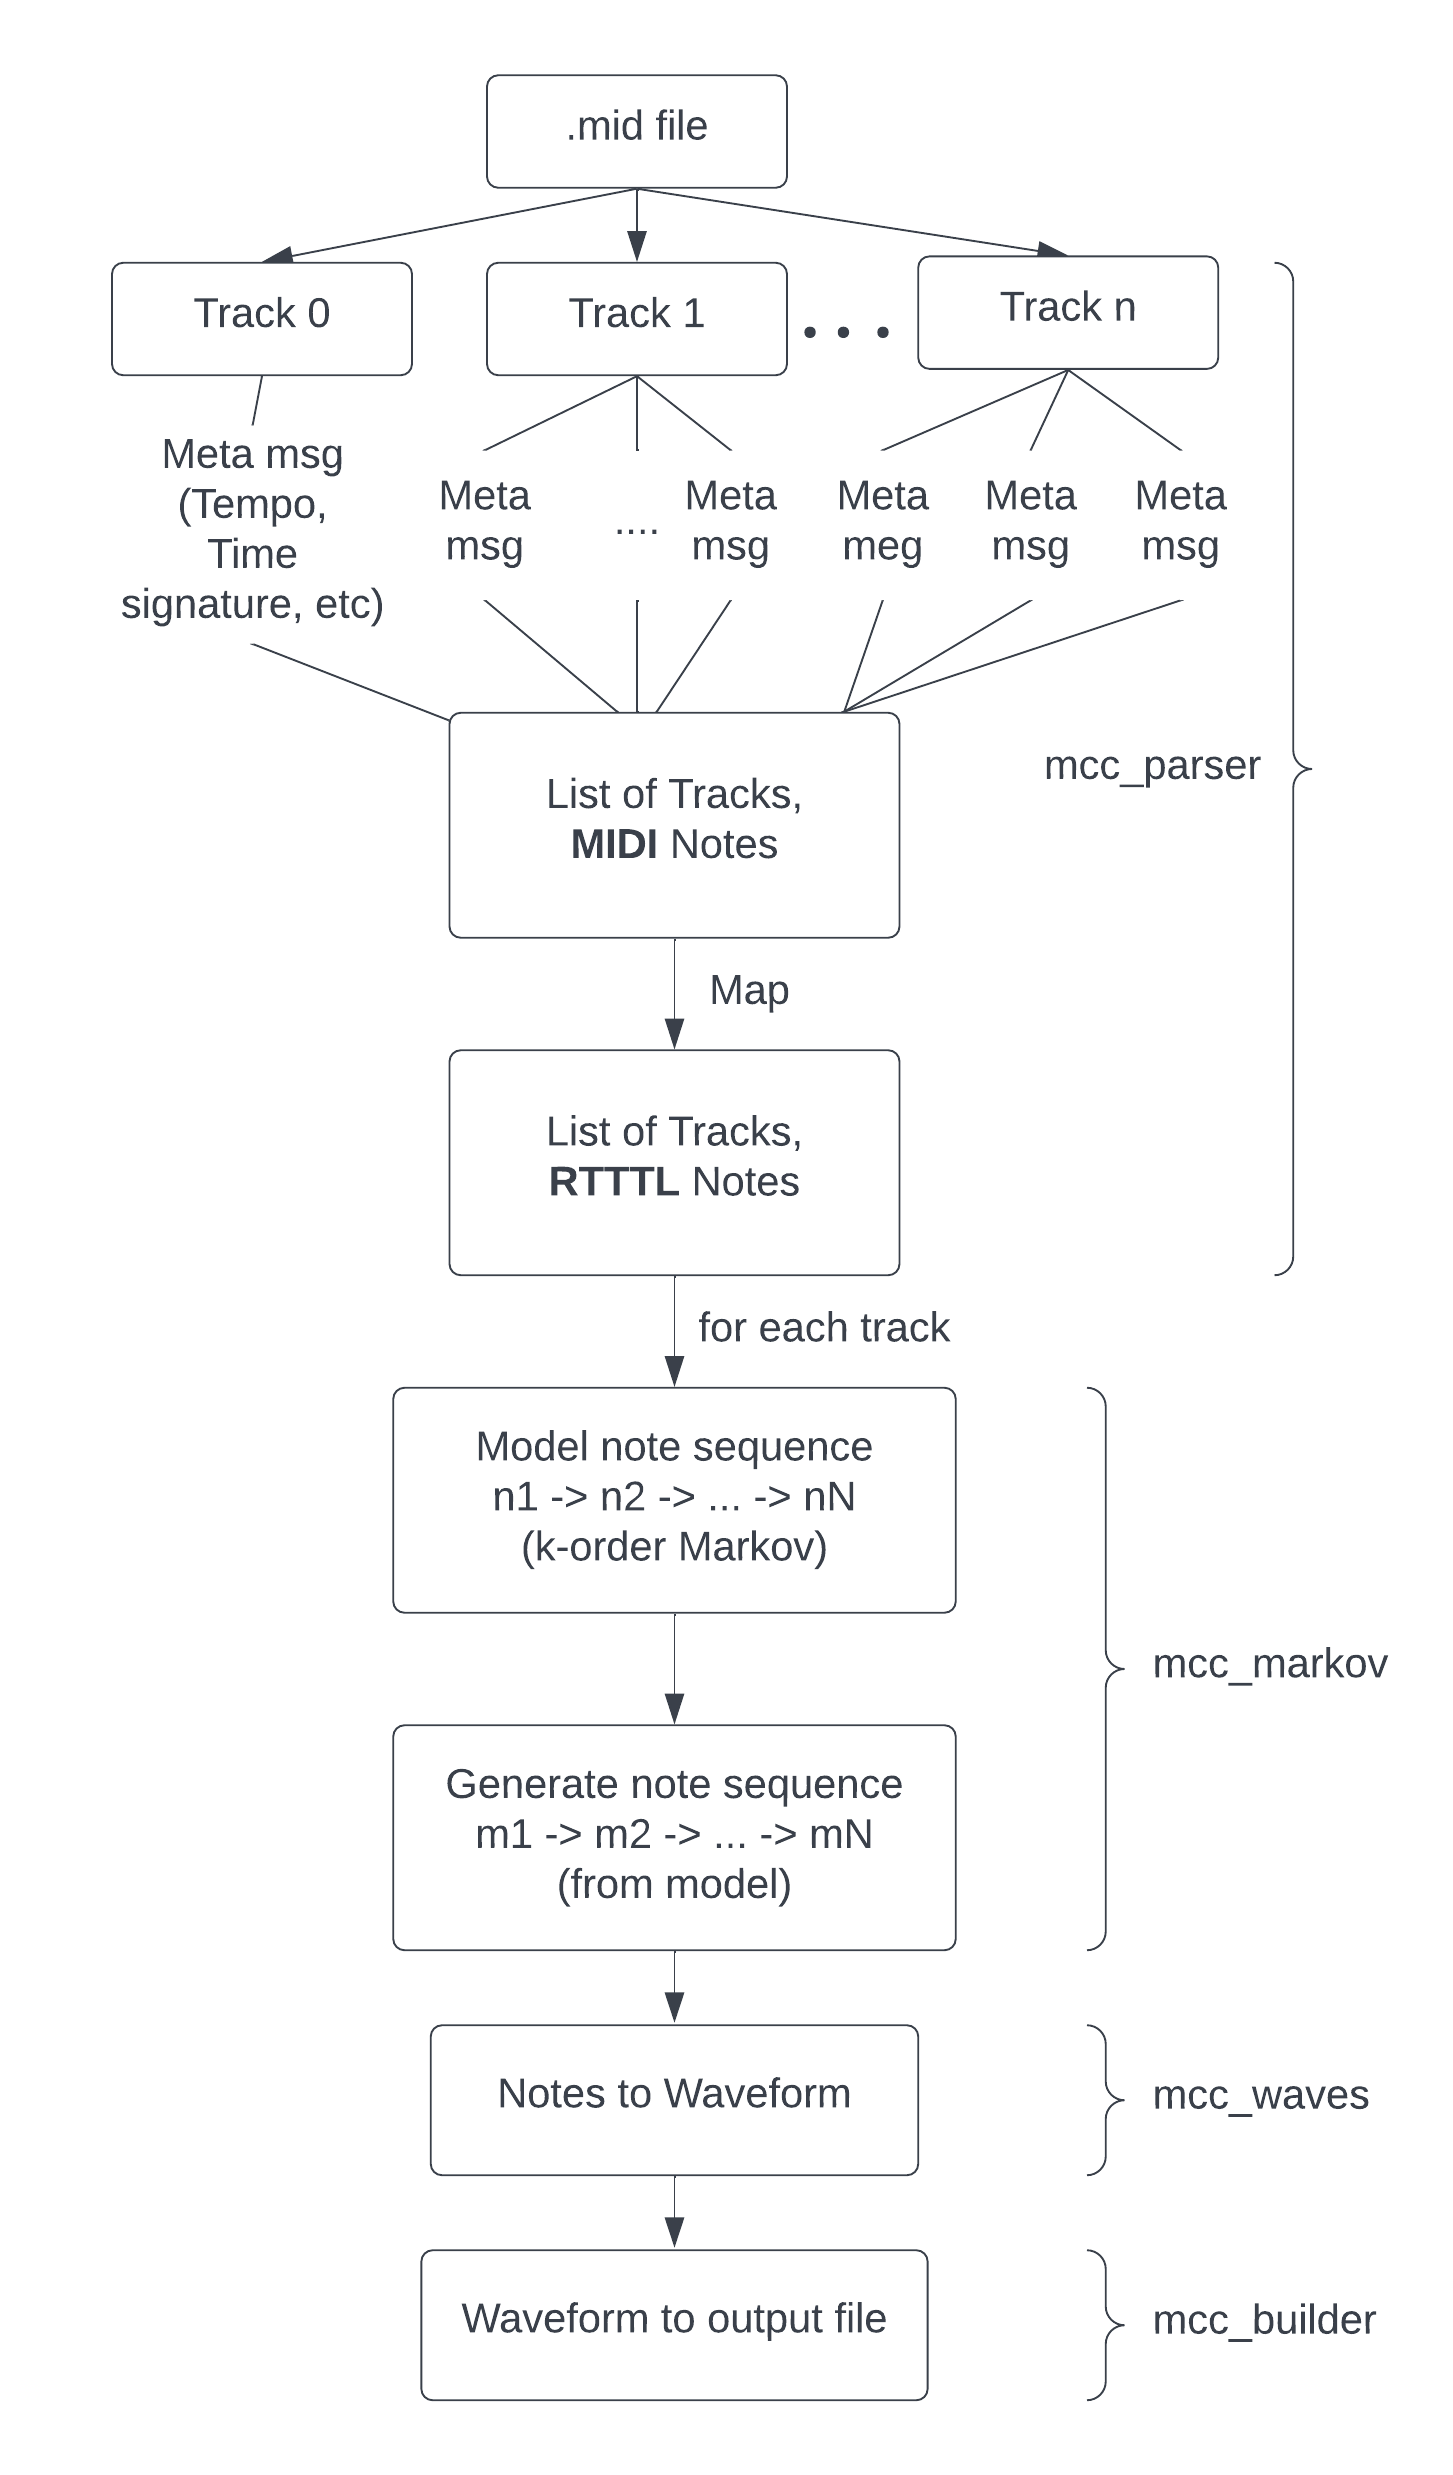
\includegraphics[width=230pt,label=Roadmap]{figs/roadmap.png}} \\

\begin{figure} 
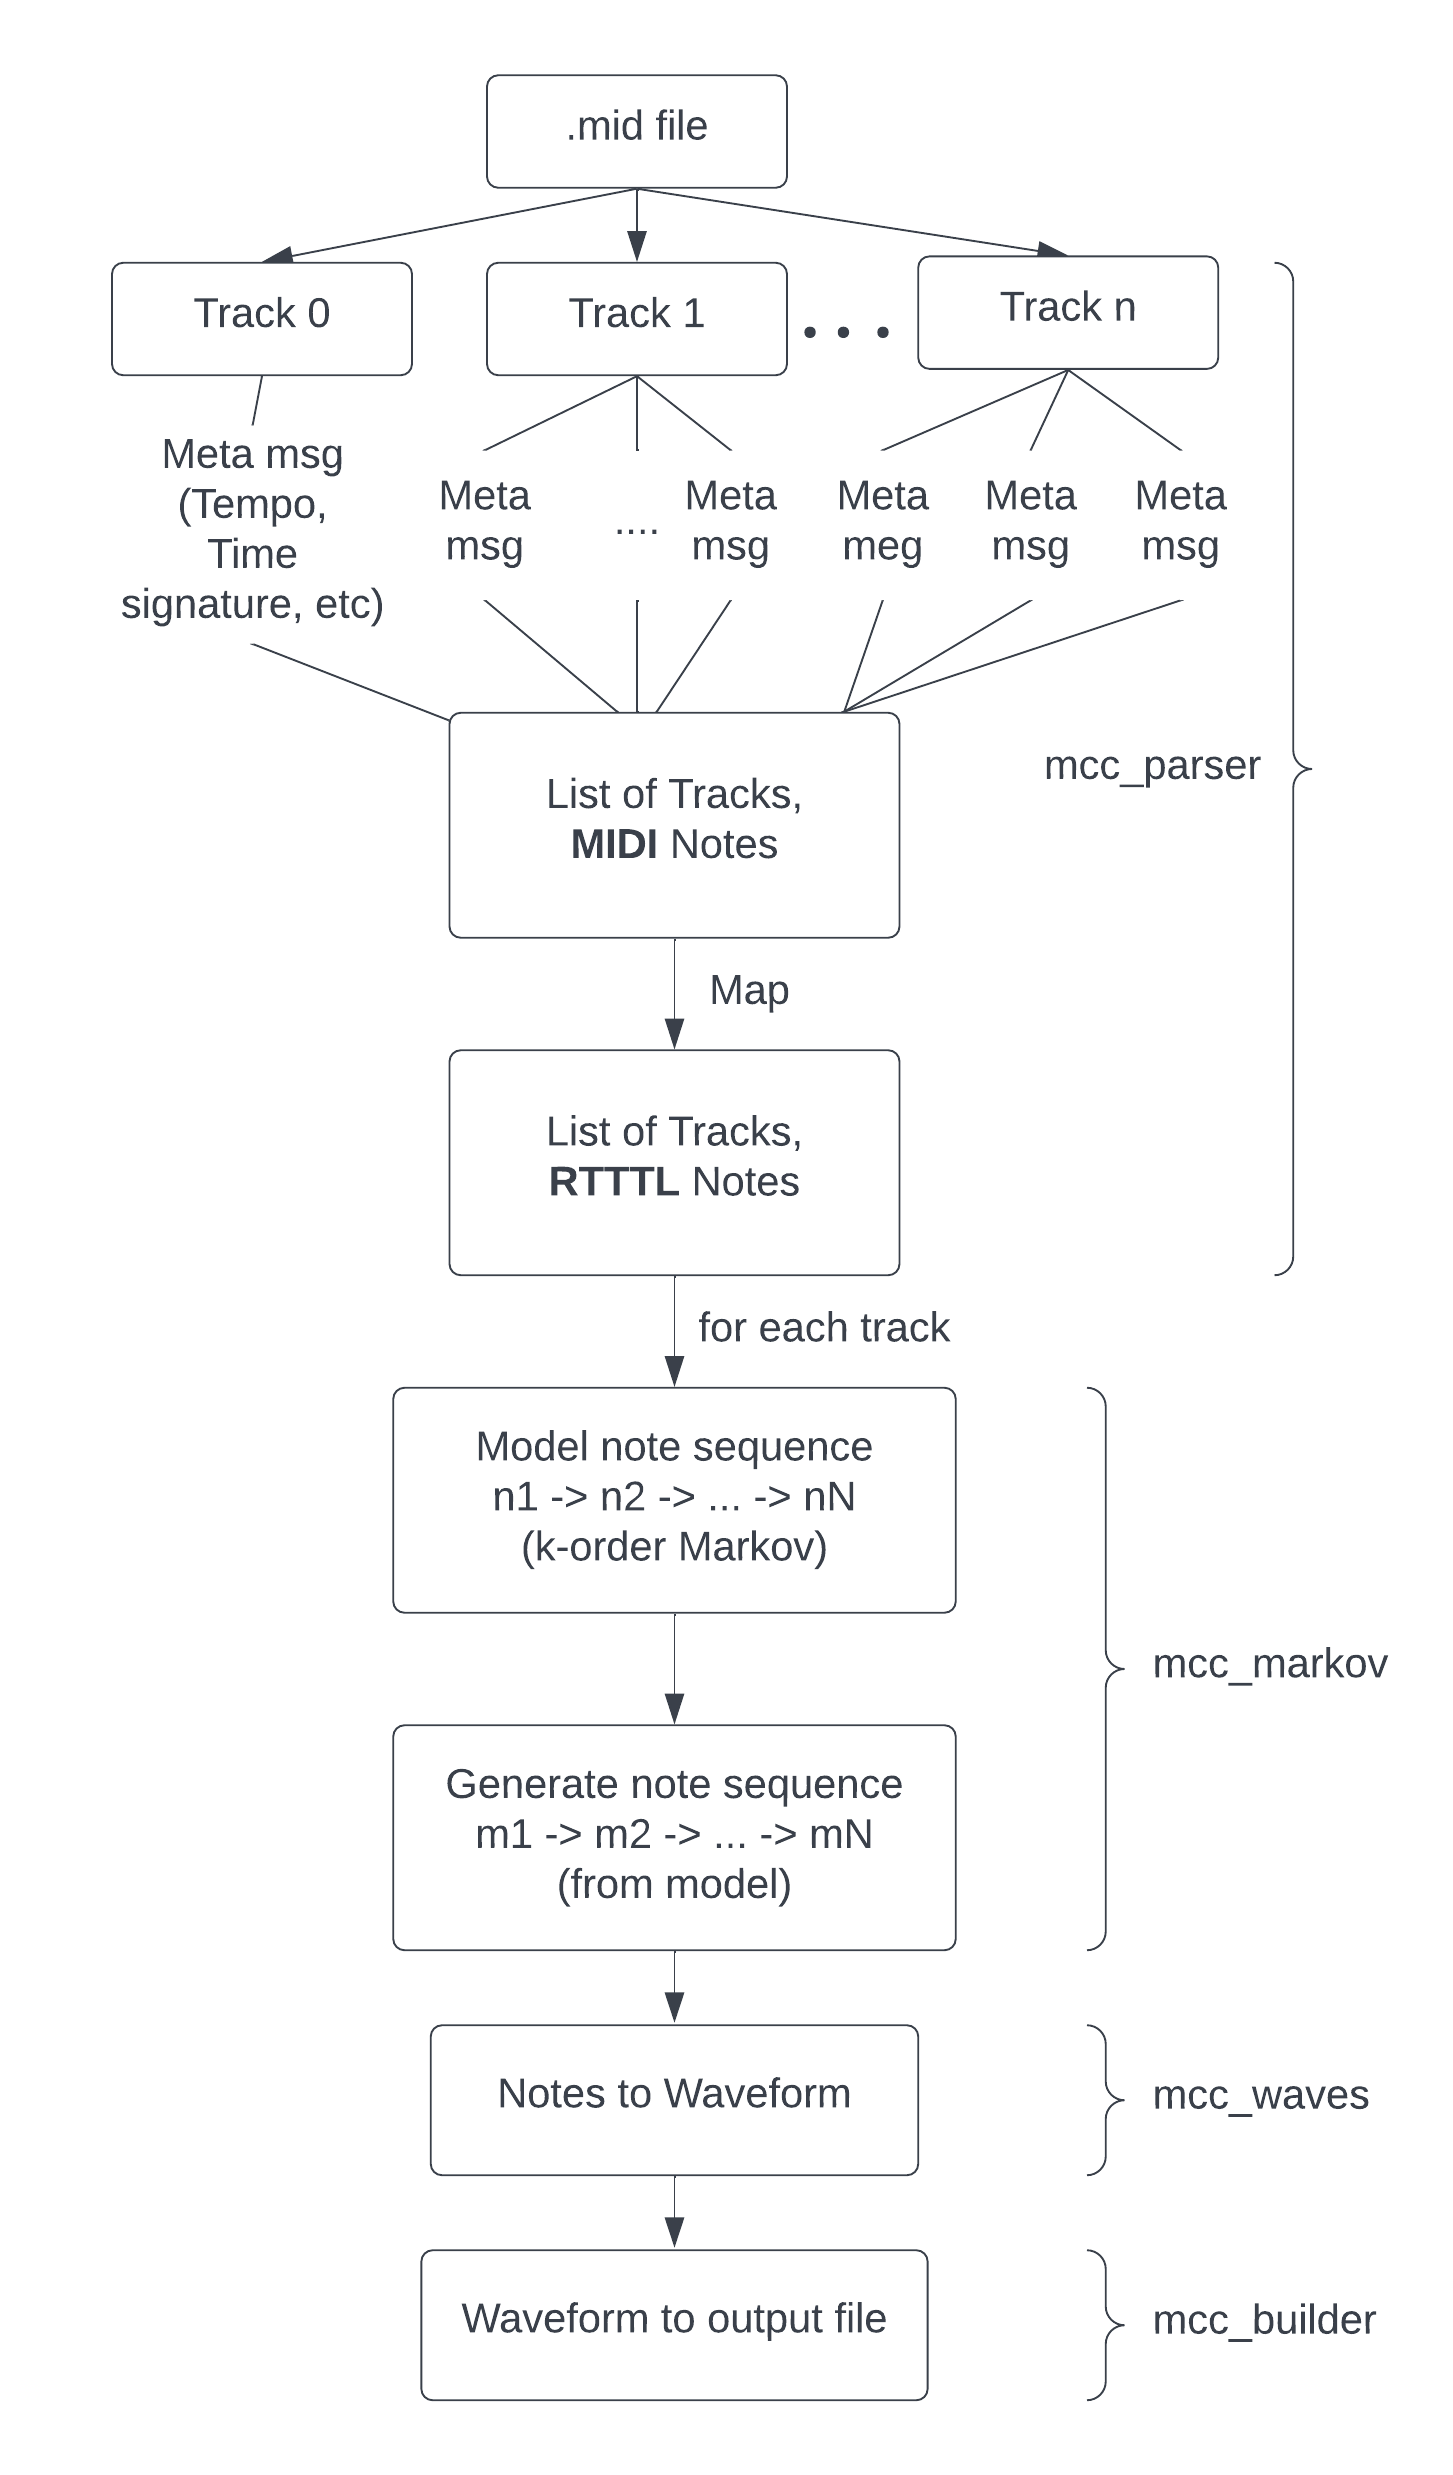
\includegraphics[width=230pt]{figs/roadmap.png} 
\caption{\small \sl The implementation pipeline.\label{fig:roadmap}} 
\end{figure} 

\subsection{Implementation}
The source code for the implementation can be found here: https://github.com/oscarsandford/chiptune-generation.

\subsubsection{MCC Parser}
The mcc-parser module parses a MID file, and converts MIDI notes to an RTTTL string. Colson worked on the most of the parser module functions, which takes a MIDI file and 
tracks as inputs, and converts them into playable RTTTL strings. Jae implemented the MIDI-to-RTTTL function, which converts each MIDI note into a corresponding RTTTL note, 
which must take into account the given beats and tempo of the song. We used some Python code we found on Github by user devxpy \cite{midi_instruments}, which converts MIDI 
note and instrument numbers to the appropriate instrument names. This function was used to attach the instrument name to each note, so that in the future, we could attempt 
to apply that instrument type to each track when generating music. 

\subsubsection{MCC Markov}
Oscar wrote two classes for Markov models in the mcc-markov module.
\begin{itemize}
  \item $SimpleMarkov$ is a naive construct for only modelling first-order Markov processes, as well as biasing the probability of the most likely action with a 
  greedification factor $\varepsilon$. 
  \item $KMarkov$ is designed to model first- and higher-order Markov processes, and is far more configurable and accurate in its output than $SimpleMarkov$ models. 
  Its success has reduced $SimpleMarkov$ to a stepping stone - a viable, but less capable solution.
\end{itemize}

Both classes have two methods: 
\begin{itemize}
  \item \textbf{Fit}: takes a sequence of states as an argument, and builds a suitable model.
  \item \textbf{Predict}: samples a fitted model for a given number of samples $n$.
\end{itemize}

While both classes are implementated generically (i.e. they can take most hashable Python types as states), they are designed to model sequences of RTTTL notes as states. 

Each track of a MIDI file is modelled as a separate chain, and sampled independently. 

Higher-order Markov chains (i.e. $k>2$) generate reasonably good-quality music that, with a high enough $k$-value (e.g. $k>50$), come to resemble the original track. By itself, 
a single extended RTTTL track may not sound great, but we assume that once we gather all the MIDI tracks in a file and combine them all, the quality of the music will be much 
better. 

\subsubsection{MCC Waves}
This module is relatively simple at a high level. It offers functionality to create square and triangle waves, as well as create ADSR envelopes for notes.

\subsubsection{MCC Builder}
The next step would be to combine tracks after generation. This is what the mcc-builder module is designed to do. Issues occur with the starting times of each track. 

All of the MIDI tracks we have collected are type 1, which means they have multiple tracks with notes, but they all start simultaneously. The way the time attribute works in 
MIDI files is that it is a reference of time elapsed from the previous message, rather than a time of that message being played. In other words, A message with $time = 0$ 
starts immediately, and the following message that has $time = 100$ plays 100 ticks (MIDI units of time) after the previous message. Herein lies the issue with multiple tracks. 

Often the melody, harmony, bass, and so forth, don't play immediately when the track starts. This causes an issue when combining the generated tracks back together, as the 
starting time is not saved anywhere. A solution we will explore is to look at the first message of each track and analyze the time value. This value can be converted to 
seconds, and saved as a value for each track. After generating the notes for each track, that value can be attached at the start, so that each track picks up at the same 
appropriate start time. 

We have completed a WAV export function for mcc-builder, which converts the sound data into a WAV file. After all those above tasks are over, If we have time, we would like 
to implement a GUI as well, as it can makes the experience more intuitive for an end-user. 

\subsection{Reflection}
Communication within the team was well done. After task delegation, each team member mostly worked on each of their task individually. Whenever someone was stuck or had 
a question, there was another person who could help out. We made steady progress as well, which is why we are keeping up with the deadlines that we set up initially. We 
expect to at least complete our project's "expected" goal by the end of the semester. See below.

One challange that we faced was the format of MIDI file was not so intuitive. Especially, the time attribute is not the time for that given message, rather, it represents 
time elapsed since the last note. We found some conflicting documentation on this matter, causing roadblocks of confusion. In order to achieve our goal, we had to make some 
compromise when parsing the MIDI notes, such as ignoring overlapping notes. Another challenge was we did not make a lot of progress during the reading break, due to 
copious reading, as well as playing video games.

The followings are our scenarios for possible outcomes:
\begin{enumerate}
  \item \textbf{Basic/minimum}: single track RTTTL notes to chiptunes generator/extender. (Accomplished!)
  \item \textbf{Expected}: MIDI file input of chiptune music with multiple tracks, generates and extends each track, outputs a WAV.
  \item \textbf{Stretch goal}: tunable model with GUI.
\end{enumerate}


\section{Evaluation}
$SimpleMarkov$ chain can process extending process very quickly. However, often the quality of the generated music was not optimal. This is because $SimpleMarkov$ is limited to 
modelling the one-state transition of notes, and does not capture the melody as a result. 
Meanwhile, the $KMarkov$ chain method with high $k$ value is slower than $SimpleMarkov$ chain method, but generates music that is closer to the input tracks it had modelled, 
resulting in higher quality music with tunable variation. We have found out that even the second order $KMarkov$ chain generates a significantly better music than the first 
order $KMarkov$ chain. We also found that the quality of the extented music sometimes depends on the specific MIDI file we chose to use.
For example, when we use \texttt{d1trans.mid} as the input, the generated music was very off-sync. But tracks such as \texttt{takeshi.mid} or \texttt{Smbtheme.mid} would 
produce music that sound more natural and enjoyable. Based on our testing, $k=3$ Markov seems to be a good balance of generating music that is derivative enough from the 
original as well as not unpleasantly random, while not being extremely time intensive.

Figure \ref{fig:stats} captures basic performance statistics for the average fit time (time to train), prediction time (time to generate notes), and 
generation time (time to convert notes to waveforms). The plots on the right hand side measure the effect of the $k$ value in $KMarkov$ with a fixed number of samples at 25. 
The $k$-value is incremented by 3 from $k=1$ to $k=100$. The plots on the left hand side measure the effect of the number of samples with a fixed $k=5$. The number of samples 
is incremented by 10 from 10 up to 500 samples. Recall that the number of samples is the number of MIDI notes that the $KMarkov$ model will generate. Computation time for 
each of these tasks is averaged across all of the songs in our data library (10 at the time of this writing, and as reflected in the plot).

\begin{figure} 
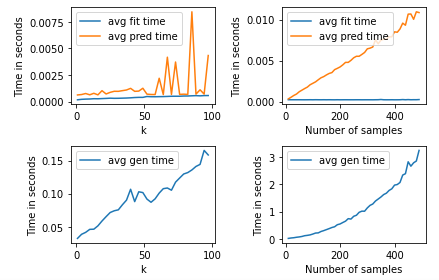
\includegraphics[width=230pt]{figs/stats.png} 
\caption{\small \sl Performance statistics relative to $k$ and the number of samples.\label{fig:stats}} 
\end{figure}

Fit time is naturally constant, independent of $k$ or the number of samples. Prediction time appears to be relatively sensitive to the $k$-value, and, as expected, linear 
with respect to the number of samples. Wave generation is more or less linear with respect to $k$-value. However, it appears that the number of samples begins to have a 
sharper and sharper impact on waveform construction time as the number increases.

\subsection{The RTTTL Tradeoff}
While the RTTTL string format is easy to work with due to its simplicity, that also comes at the cost of precision - there is no free lunch. We found that the current method 
we used for generating the appropriate rest betweeen notes is not flawless. The assign-note function in mcc-parser is responsible for returning the appropriate note lengths 
and rest lengths for RTTTL notes. However it only returns discrete values, as that is what is required of RTTTL. What this means is that if the result is at the upper end of a 
range, it gets set to the lower value. This can cause the wrong values to be set for notes and rests, which throws off the synchronization of the tracks when combining them. 
In the future, fixing the note length creation would cause generated music to sound more like the original, and be more in sync.

\subsection{GUI Development}
For demonstration and usability purposes, we have implemented a GUI as well. It is a simple media player based on Israel Dryer's Media player project. We previously tried 
to implement a GUI using TKinter and Pygame. However, the generated WAV file was not playable. After extensive research, we found out that the main problem was the format 
of the WAV file. We used scipy to convert the extended music data to WAV file, and while scipy saves the WAV file as int8 format,
Pygame's media player requires int16 (or higher) format in order to play a WAV file. So instead, we decided to reference Israel Dryer's Media-Player project \cite{media_player}.
It is a simple, open source media player that uses TKinter and VLC. The author was very open to modification and extension of the project, especially for educational purposes.
We added a function and button where the user can upload MIDI file and execute the extension process. VLC was a lot more flexible in terms of file format and we were able 
to play the generated music without a problem.

% Promises of extensibility.
\section{Conclusion} 
It would be great to make our program more robust and able to handle a larger variety of songs, such that difficult MIDI message types are not impossible to extract
data from. This way we would be able to handle more dynamic songs and not be so limited in our choices. Our implementation will be maintained as an open source 
project \footnote{https://github.com/oscarsandford/chiptune-generation} in order to expand its functionality and improve its user interface. The following is a non-exhaustive 
list of planned features:
\begin{itemize}
  \item \textbf{Enhanced GUI}: Make the GUI more original and aesthetically pleasing, additional features to allow high-fidelity HCI with API.
  \item \textbf{Solve syncing issue}: Fix issue of tracks not playing in sync after generation.
  \item \textbf{Note-waveform mappings}: Use existing MIDI instrument labels to map notes to different types of waveforms.
  \item \textbf{Make mcc-parser more robust}: Ensure program can handle more complex MIDI message types without failure.
  \item \textbf{Make waveform generation more efficient}: Use caching and explore other methods to reduce computation time in generation waves.
  \item \textbf{Explore methods for quantitative evaluation}: Experiment with cross-similarity matrices as a way to evaluate replication accuracy instead of only measuring 
  generation quality through qualitative analysis. 
\end{itemize}
Overall, we were able to learn a lot about the chiptune music genre and different ways to extend it. As this project is an open sourced project, we would like to encourage
anyone who has passion in chiptune music or music extension using Markov chains to participate and expand the horizon of this project.
% END

% Add bibtext citations to the file `refs.bib`.
\bibliography{refs}
\end{document}
